\documentclass{article}

% formatting
\usepackage[utf8]{inputenc} % allow utf-8 input
\usepackage[T1]{fontenc} % use 8-bit T1 fonts  (allows for direct use of ö,ü,etc.)

% math typesetting
\usepackage{amsmath}
\usepackage{amsfonts}

% color
\usepackage{color}
\usepackage{xcolor}

% layout
\usepackage{layout}
\usepackage{lipsum}

% cross-referencing and hyperlinks
\usepackage{hyperref}
\usepackage{url}
\usepackage{doi}

% figures
\usepackage{graphicx}

% tables
\usepackage{booktabs}
\usepackage{multirow}
\usepackage{caption} 
\usepackage{float}

% enumeration
\usepackage{enumitem}

% embedding pages
\usepackage{pdfpages}

% multi-line comments
\usepackage{comment}

% footnotes
\usepackage{footnote}

\usepackage{subfig}
\usepackage{cleveref}

\usepackage[
    backend=biber,
    style=authoryear-comp
]{biblatex}
\addbibresource{references.bib}

%%%%%%%%%%%%%%%%%%%%%%%%%%%%%%%%%%%%%%%%%%%%%%%%%%%%%%%%%%%%%%%%%%%%%

% document metadata
\title{Proposal for a Summer Academy of the Swiss Study Foundation}
\author{Michael Weinold, Philippe Schultheiss et al.}
\date{2023}

%%%%%%%%%%%%%%%%%%%%%%%%%%%%%%%%%%%%%%%%%%%%%%%%%%%%%%%%%%%%%%%%%%%%%

\begin{document}

\maketitle

\section{Introduction}

\begin{figure}[]
    \centering
    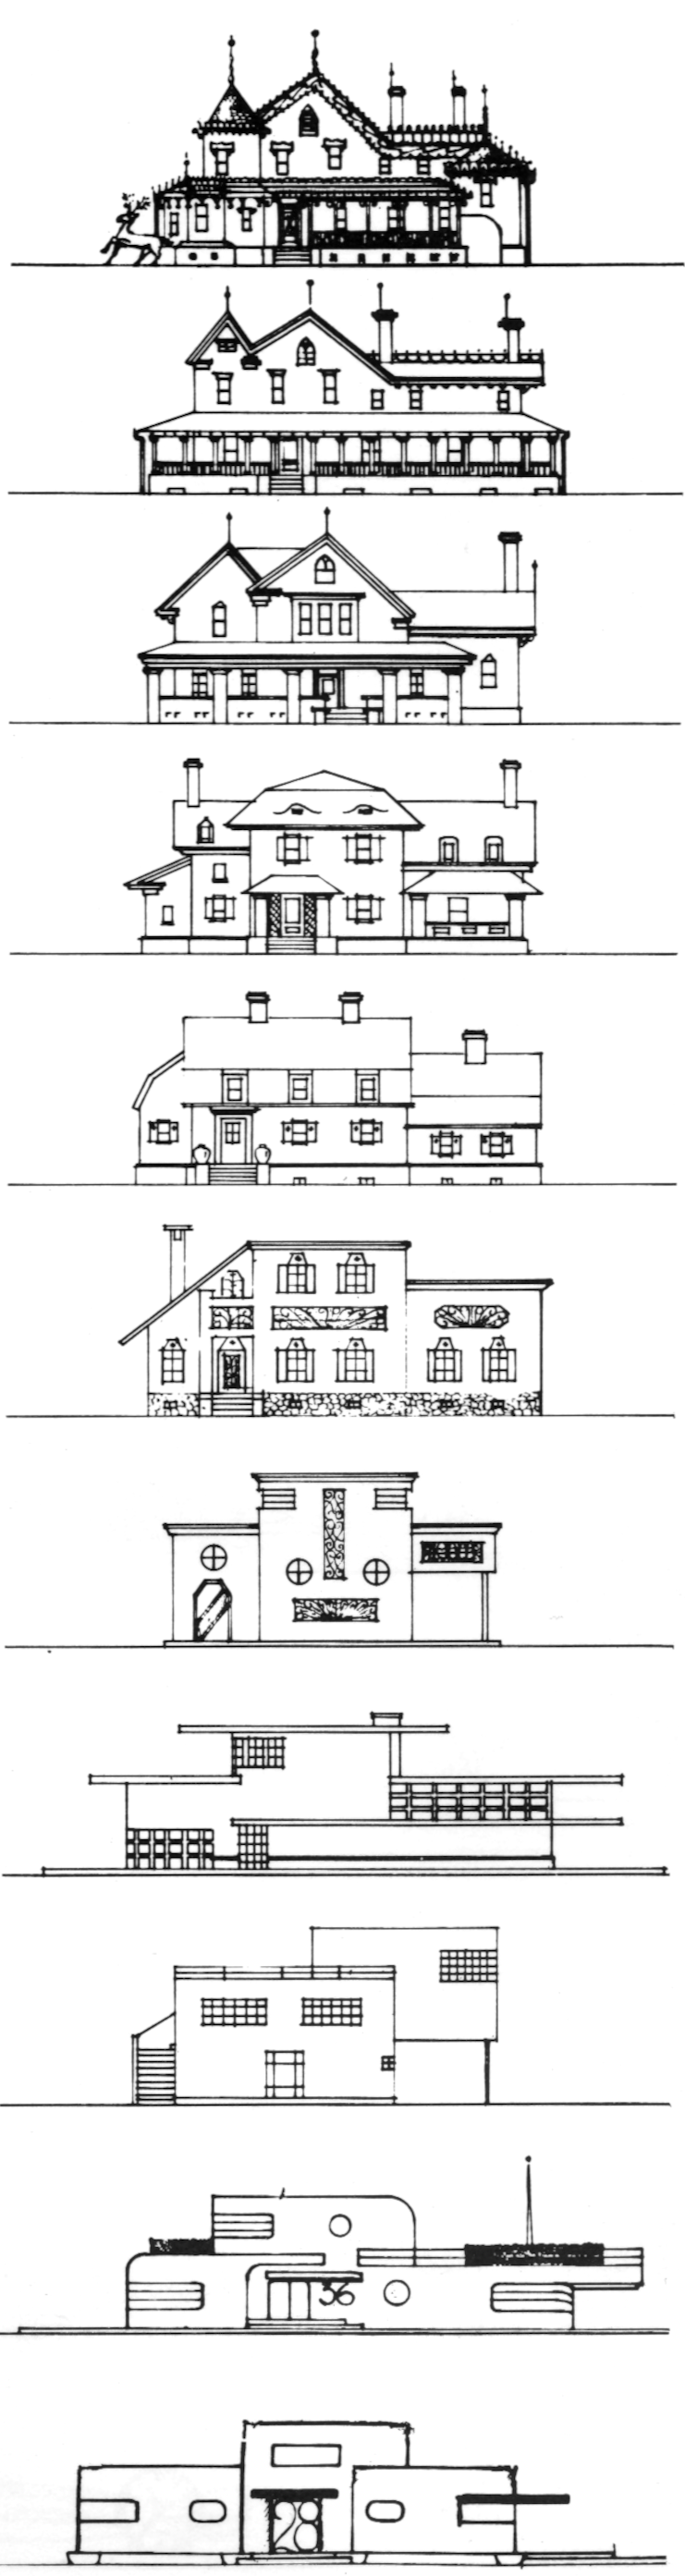
\includegraphics[height=\textheight]{./figures/loewy_architecture.png}
    \caption{
        Some text here. Source: "Design Evolution 1930", \cite{loewy_industrial_1979}
    }
    \label{fig:combined}
\end{figure}

\newpage

\begin{figure}
    \centering
    \subfloat{{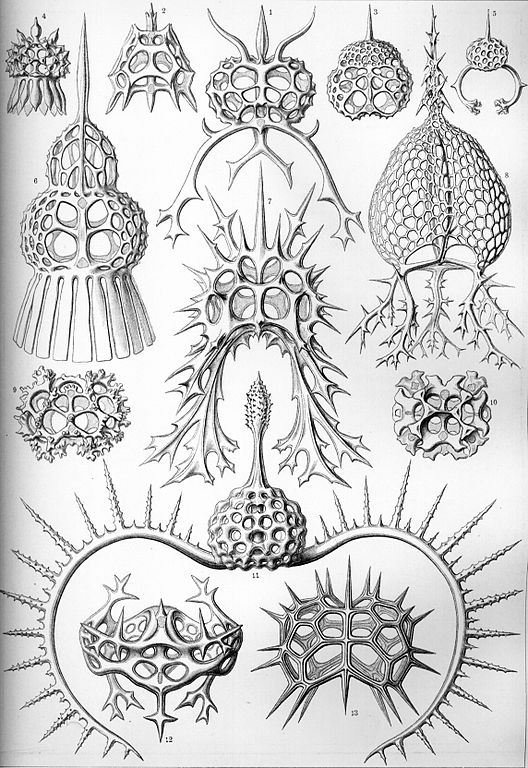
\includegraphics[height=5.5cm]{figures/Spyroidea.jpg} }}
    \subfloat{{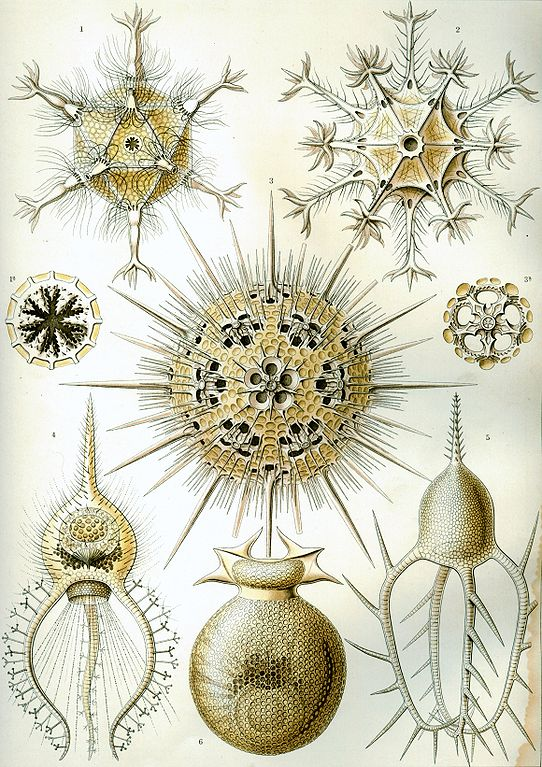
\includegraphics[height=5.5cm]{figures/Phaeodaria.jpg} }}
    \subfloat{{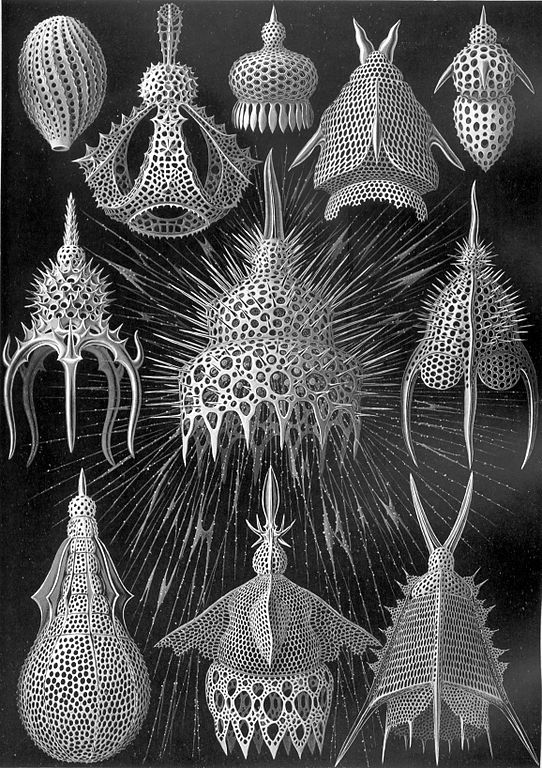
\includegraphics[height=5.5cm]{figures/Cyrtoidea.jpg} }}
    \caption{Selection of drawings from Ernst Haeckel's \textit{"Kunstformen der Natur" (en.: "Art Forms in Nature")} \cite{haeckel_kunstformen_2012}. According to Rene Binet, drawings like these served as inspiration for his monumental arch \cite[Sec. "Haeckel und der Jugendstil"]{willmann_haeckel_2019}, which is depicted in \cref{fig:arch}. Image sources from left to right: Spyroidea \cite{haeckel_kunstformen_1904}, Phaeodaria \cite{haeckel_kunstformen_1904} and Cyrtoidea \cite{haeckel_kunstformen_1904-2} by Ernst Haeckel.}
    \label{fig:kunstformen}
\end{figure}

\begin{figure}
    \centering
    \subfloat{{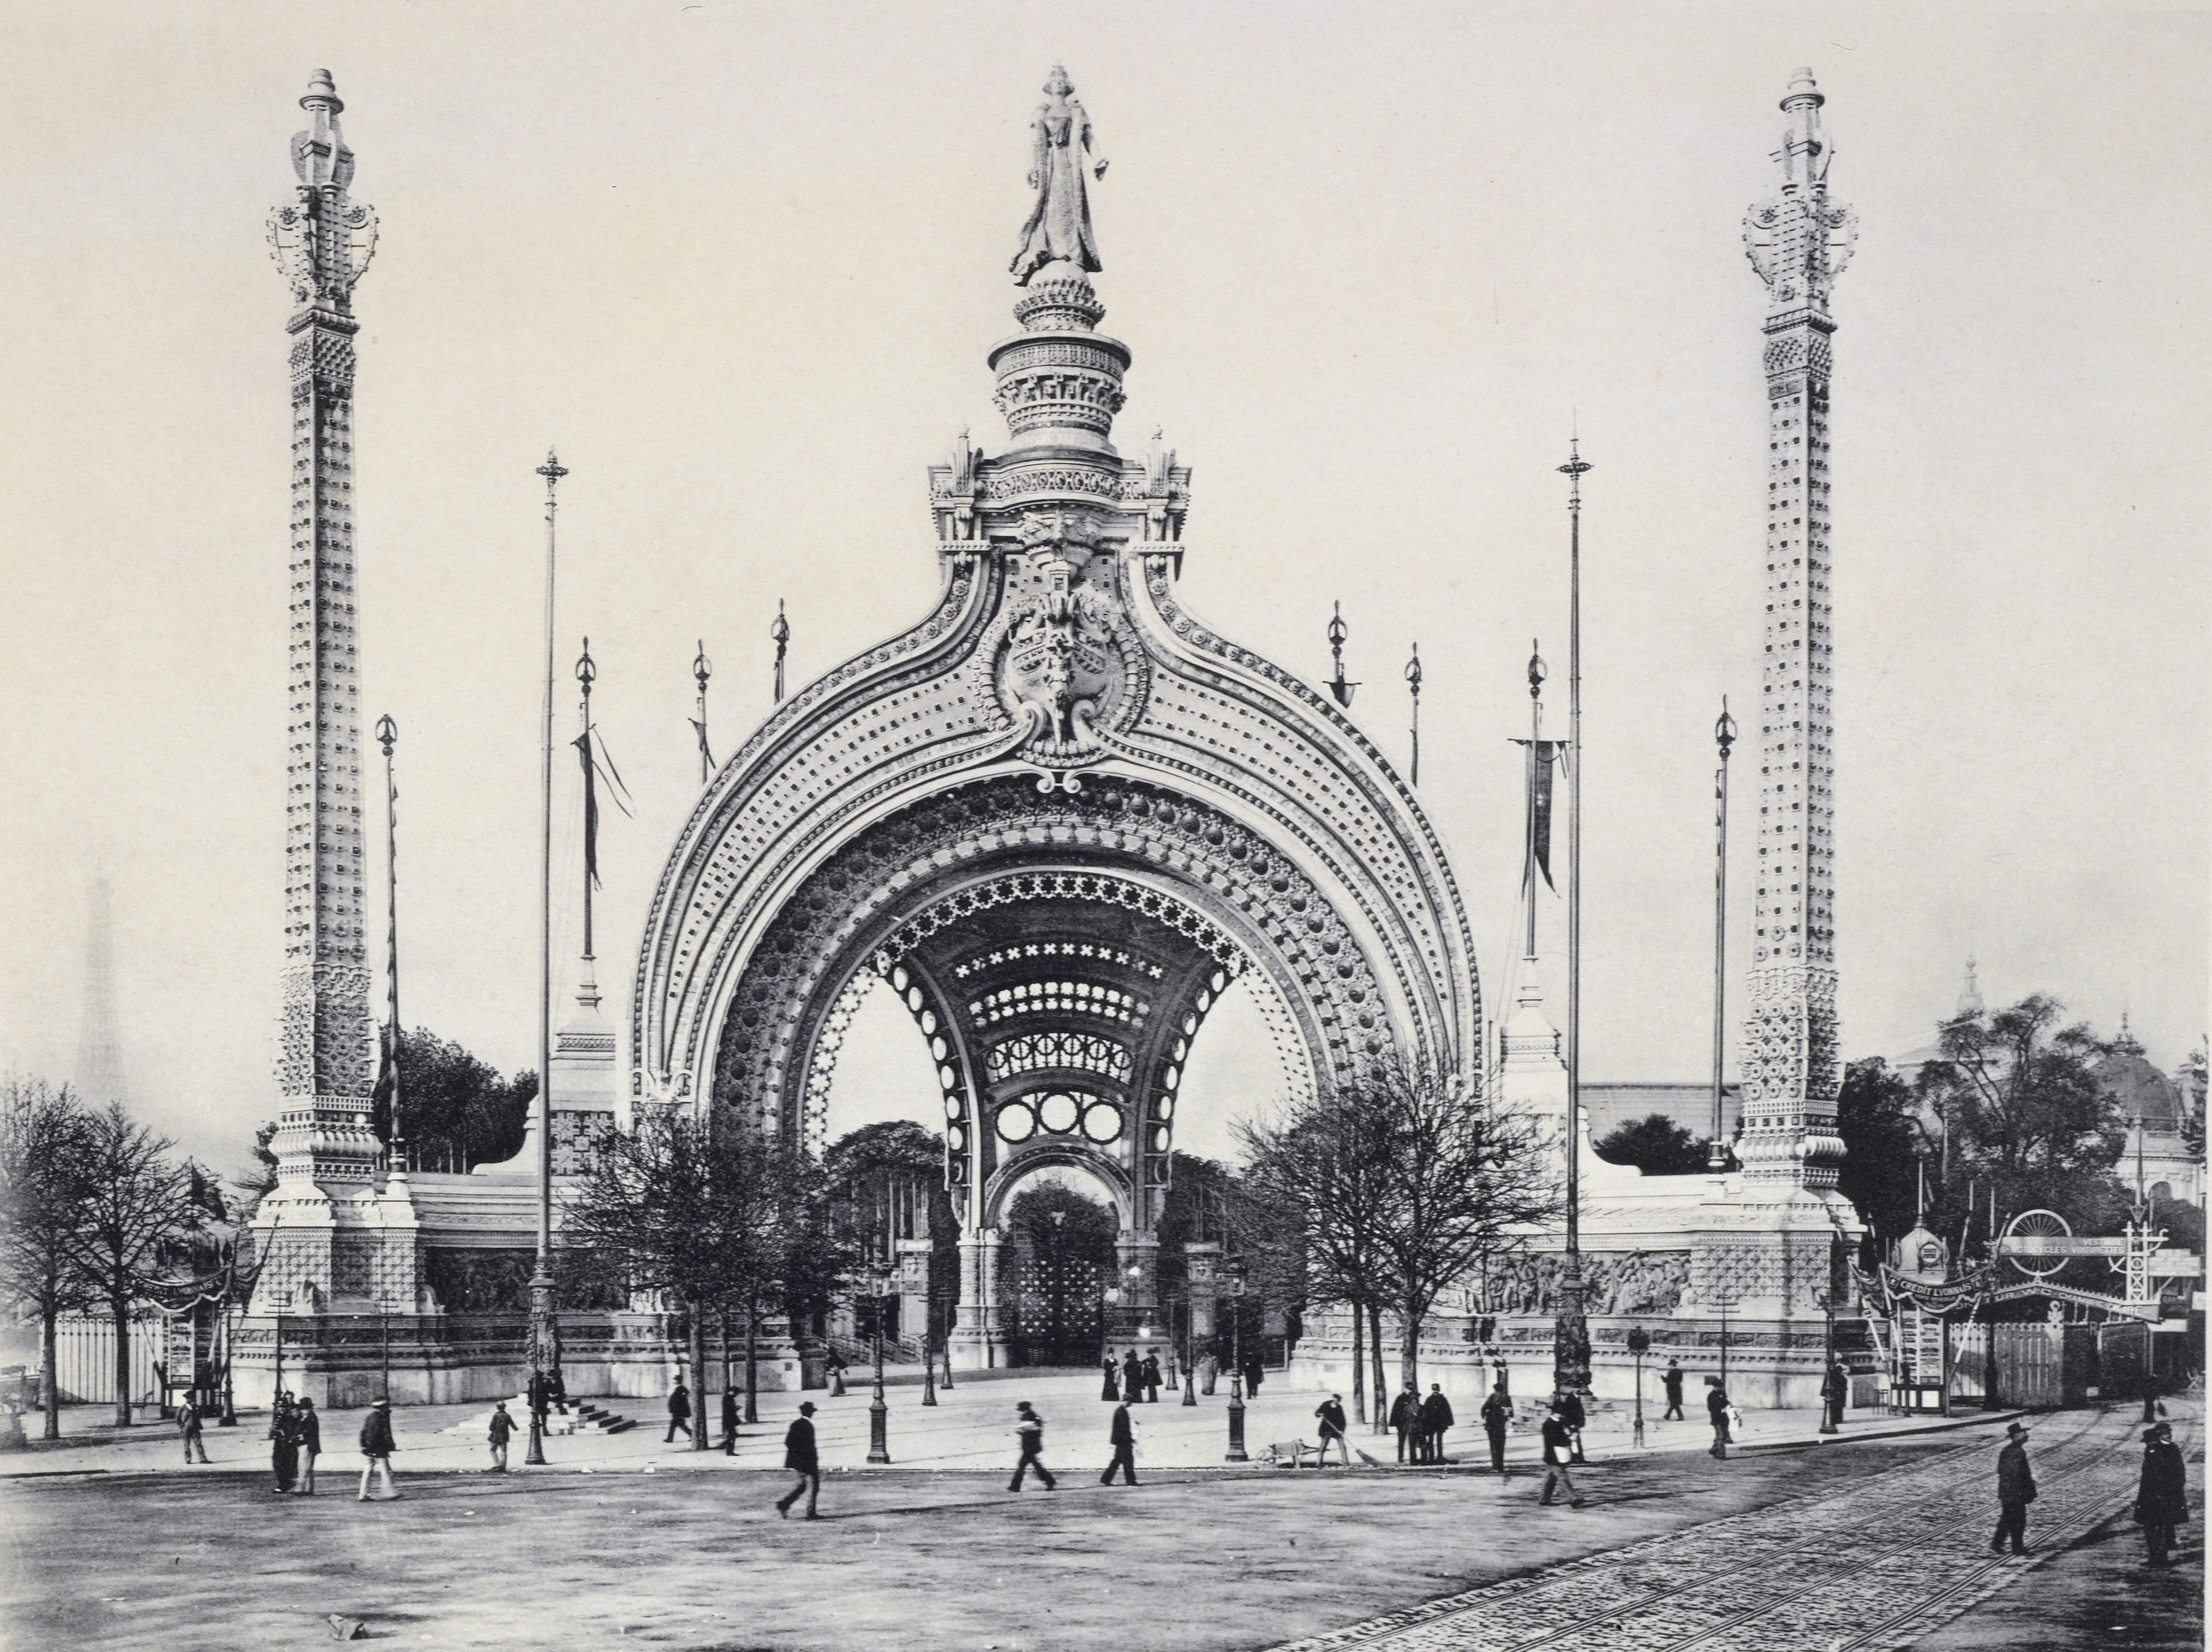
\includegraphics[height=4cm]{figures/porte_photograph.jpg} }}
    \subfloat{{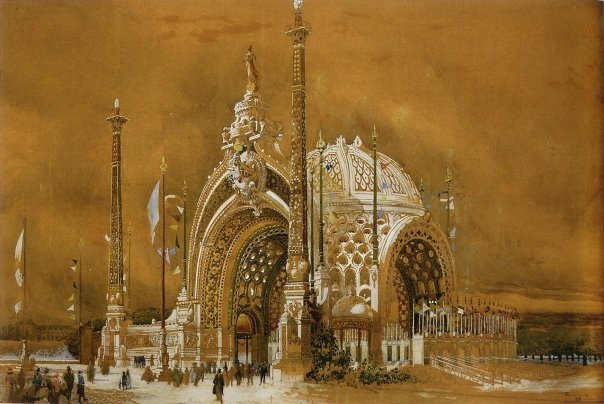
\includegraphics[height=4cm]{figures/porte_watercolor.jpg} }}
    \caption{Two renderings of the \textit{"Porte Binet"}, a monumental gate designed by Rene Binet for the 1900 Paris Exposition. Image sources: Photograph by Larger \cite{louis_porte_1900} and watercolor on paper by Binet \cite{binet_projet_1898}.}
    \label{fig:arch}
\end{figure}

\clearpage
\printbibliography

\end{document}
